\subsection{Project board}\label{sec:project-board}

One of the great tools that helped with the project management
was the new Github Projects app,
depicted in figure~\ref{fig:github-projects-kanban},
which was in beta stage
when I started to use it~\cite{github_inc_github_2022}.
The Kanban board~\cite{goddard_kanban_2022} consists of four sections (columns):

\begin{itemize}
      \item
            \textit{Todo} -- which consists of all the issues
            connected to this project
            that are planned to be worked on in the future;
      \item
            \textit{Open} -- which consists of issues
            that need to be worked on next.
            Those are usually one to three issues
            that need to be done in a certain order;
      \item
            \textit{In Progress} -- which contains issues
            that are currently being worked on.
            There is usually only one issue in this column;
      \item
            \textit{Done} -- which consists of all the finished issues,
            as well as the issues that were deemed unnecessary,
            in which case, they are labeled ``won't fix''.
\end{itemize}

Another convenient tool in the same Github Projects app
was the table view.
I~configured one of the table views to present a Backlog,
a list of issues in the whole project,
which I could manually sort by
issue priority and urgency
so as to enable quick progress overview.
The Backlog view is presented in figure~\ref{fig:github-projects-backlog}.

\begin{figure}[!h]
      \centering
      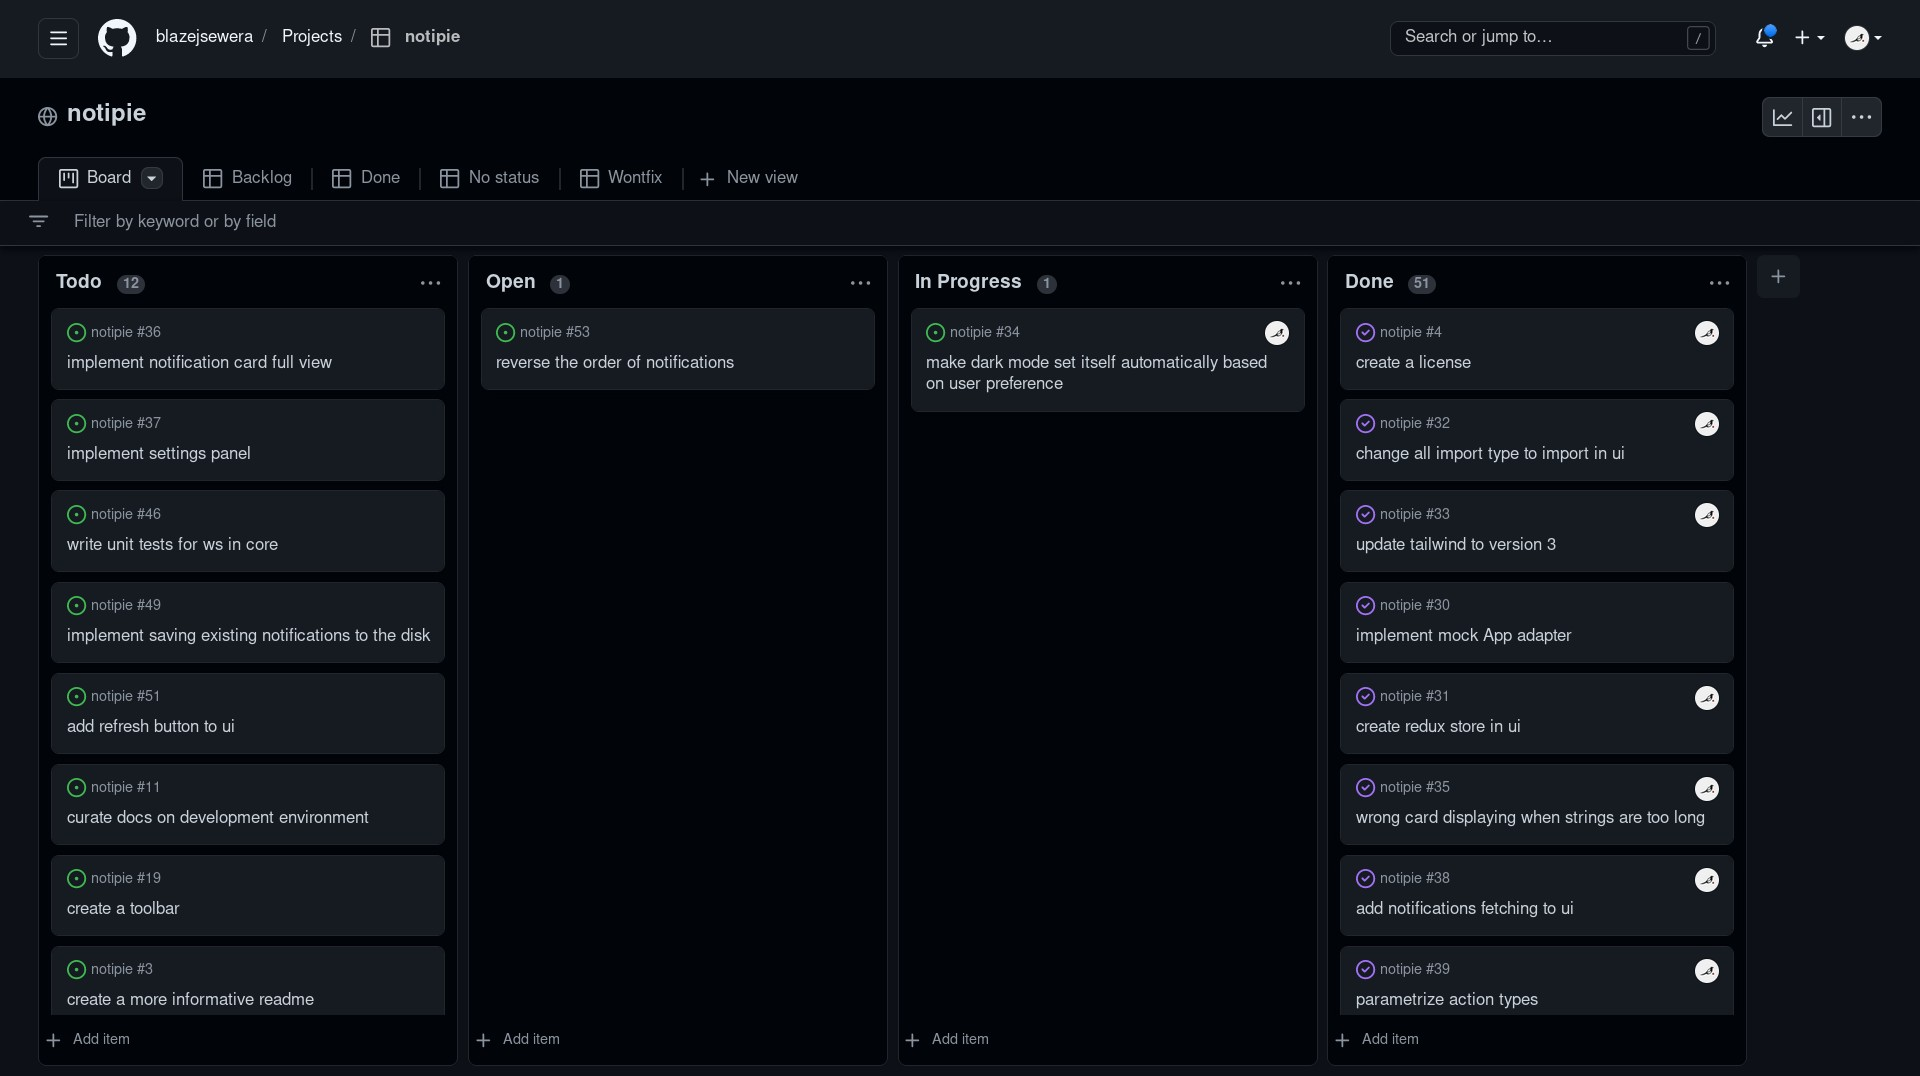
\includegraphics[width=0.99\linewidth,keepaspectratio]{img/kanban_board.jpg}
      \caption{Github Projects: Kanban board view}
      \label{fig:github-projects-kanban}
\end{figure}

\begin{figure}[!h]
      \centering
      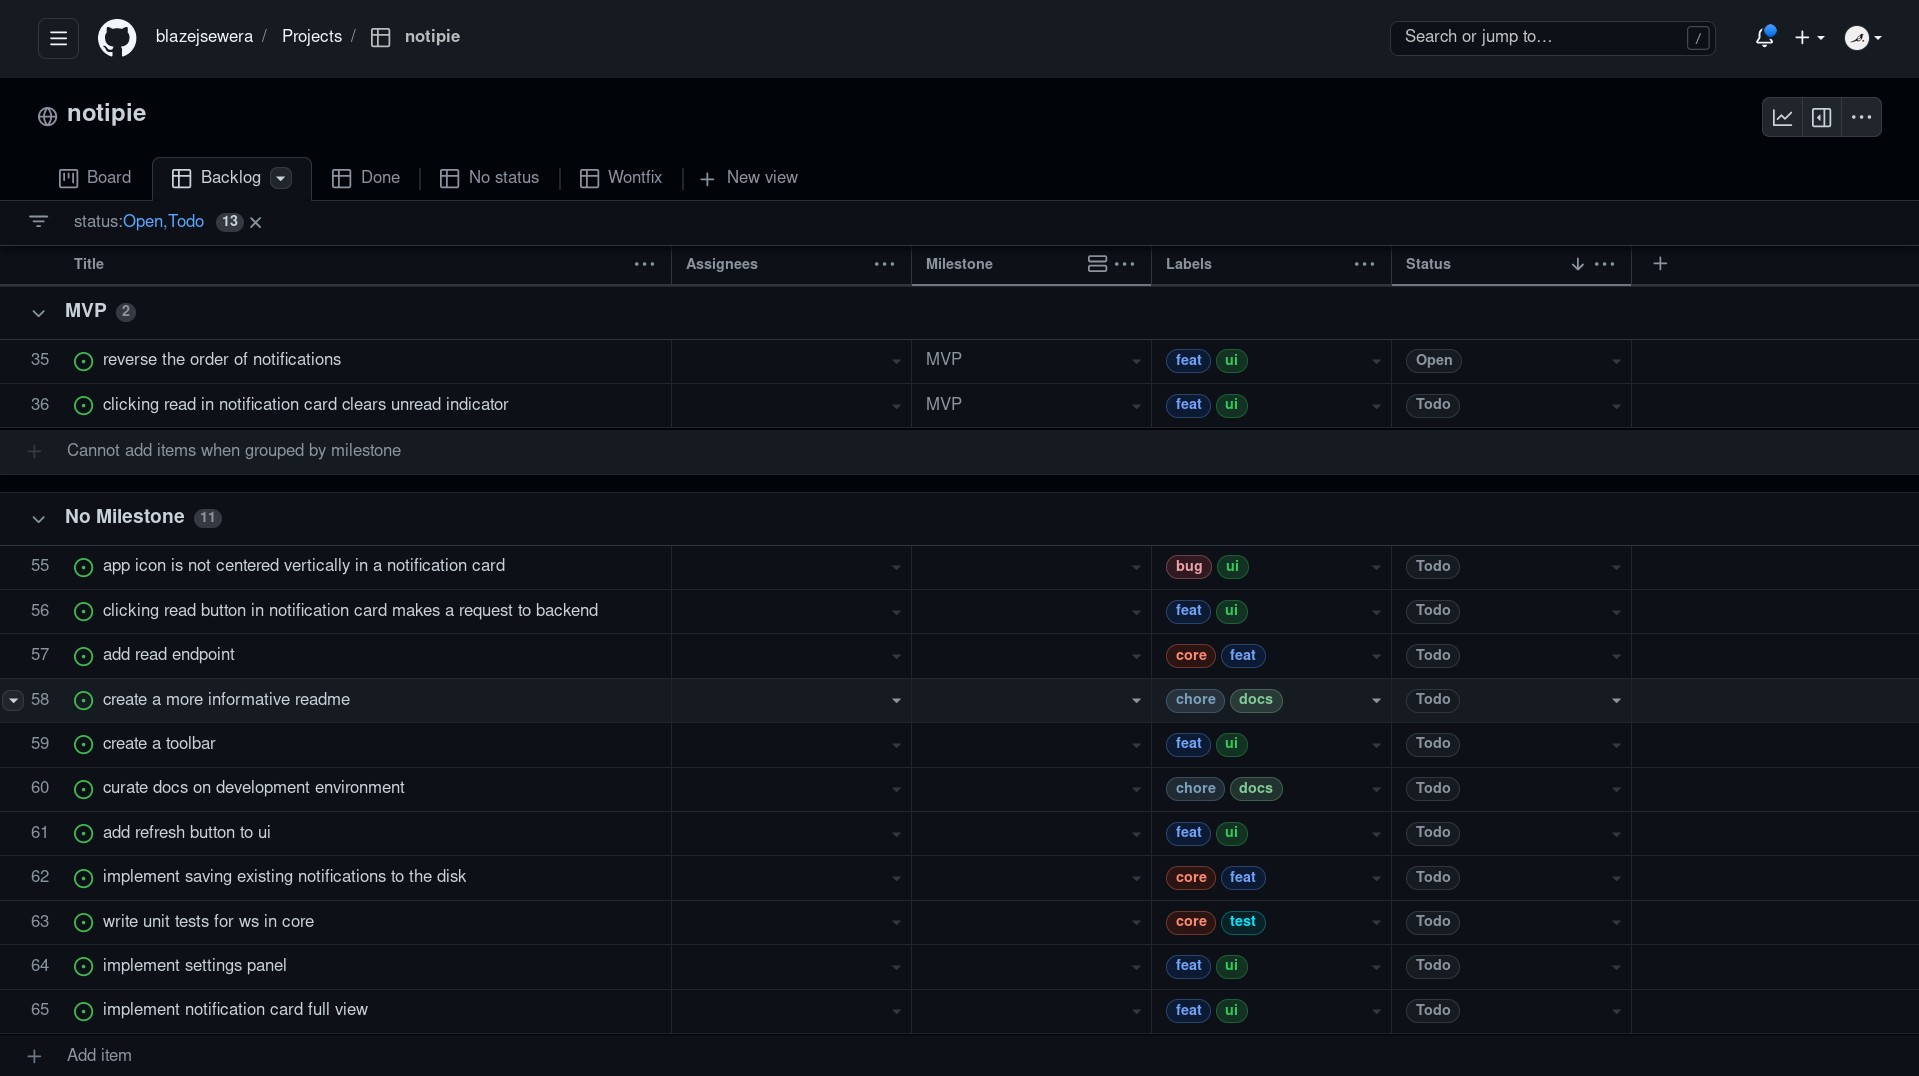
\includegraphics[width=0.99\linewidth,keepaspectratio]{img/backlog.jpg}
      \caption{Github Projects: Backlog view}
      \label{fig:github-projects-backlog}
\end{figure}
